Med ett svep på $50~\textrm{V}$ accelerationsspänning, $U_A$, gavs följande vy, \Cref{fig:ollle} och värdena i \Cref{tab:maxmin}.
\begin{figure}[h]
	\centering
	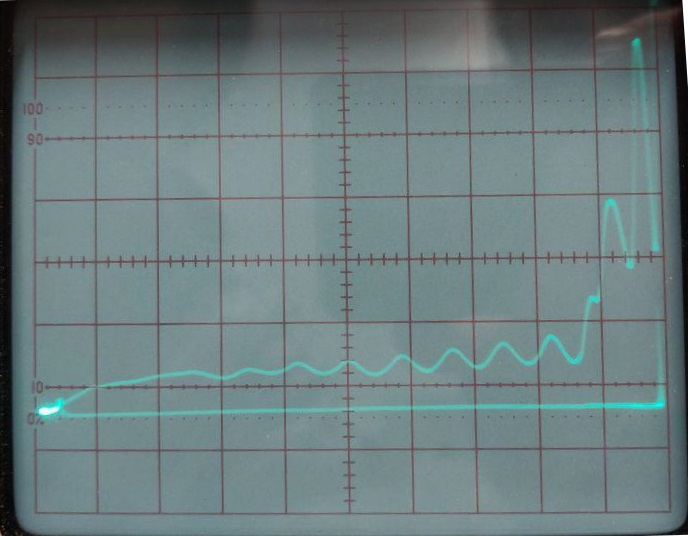
\includegraphics[width = .8\textwidth]{osc_light_low_lowUA_e.jpg}
	\caption{x-led: accelerationsspänning, $U_A$, [$5~\textrm{V/Major div.}$]\\
			y-led: ström, $I_A$, [arbiträr enhet]}
	\label{fig:ollle}
\end{figure}

\begin{minipage}{\linewidth}
\begin{table}[H]
\centering
	\begin{tabular}{llll}
 	\textbf{Maxima [div.]}& \textbf{Maxima [V]}&\textbf{Minima [div.]}& \textbf{Minima [V]}\\\hline
	$3.4$&$17$&$3.0$&15\\
	$4.2$&$21$&$3.8$&19\\
	$5.0$&$25$&$4.6$&23\\
	$5.8$&$29$&$5.4$&27\\
	$6.6$&$33$&$6.2$&31\\
	$7.4$&$37$&$7.0$&35\\
	$8.2$&$41$&$7.8$&39\\
	$8.8$&$44$&$8.4$&42\\
	$9.0$&$45$&$ - $&
 	\end{tabular}
\caption{Maxima och minima i [divisioner] (för jämförelse mot graf) och [V] för analys. Data utläst från graf \cref{fig:ollle}}
\label{tab:maxmin}
\end{table}
\end{minipage}
\vspace{.5cm}

Från \Cref{fig:ollle} kan det ses hur strömmen ökar exponentiellt med högre accelerationsspänning med periodiska dipp som motsvarar excitationsenergierna för kvicksilver, 4eV, enligt periodiciteten som ses i \cref{tab:maxmin}. Den exponentiella ökningen ses tydligt i början av \Cref{fig:dark_high} där vi testade extremerna för systemet.
% TODO: "där vi testade extremerna för systemet" låter för ospecifikt tycker jag. Läsaren kommer ju inte ha någon aning om vad vi menar. 

Från jämförelse mellan bilderna \cref{fig:dark_lowub,fig:dark_highub} kan vi se att en skillnad i spänningen över filamentet ``förskjuter'' området vi ser maximan och miniman. I cref{fig:dark_highub}, där $U_b$ har ökats, syns de periodiska fallen i strömmen bara mot slutet av skalan, där accelerationsspänningen är stor nog för att driva elektronerna förbi potentialbarriären. 
%Filament voltage effect:
%Scales up or shifts current earlier along the acceleration voltage axis.

\begin{figure}[h]
	\centering
	\begin{subfigure}[c]{0.47\textwidth}
	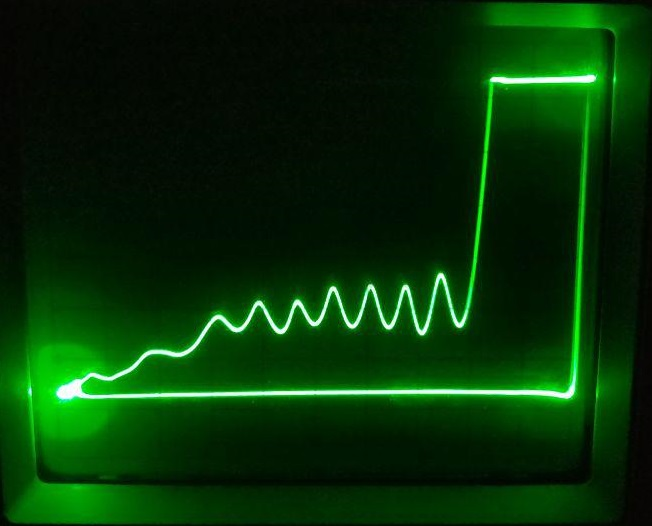
\includegraphics[width=\textwidth]{osc_dark_low_lowUA_e.jpg}
	\caption{Utströmmen mot accelerationsspänningen då en låg backspänning lagts på. Dalarna motsvarar de kinetiska energier varvid elektronerna stoppas av och exiterar kvicksilveratomerna.}
	\label{fig:dark_lowub}
	\end{subfigure}
	~
	\begin{subfigure}[c]{0.49\textwidth}
	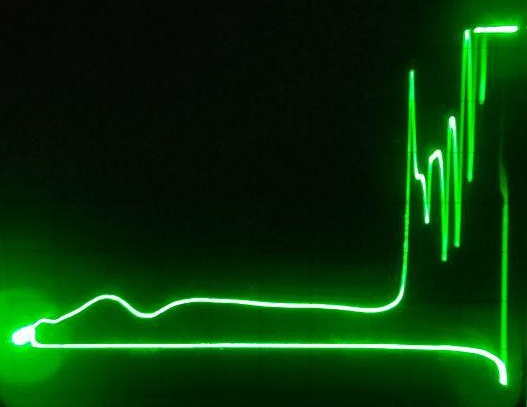
\includegraphics[width=\textwidth]{osc_dark_low_highUA_e.jpg}
	\caption{Efter backspänningen ökat krävs det mer accelerationsspänning för att nå anoden och registrera som ström.}
	\label{fig:dark_highub}
	\end{subfigure}
	
	\begin{subfigure}[c]{0.47\textwidth}
	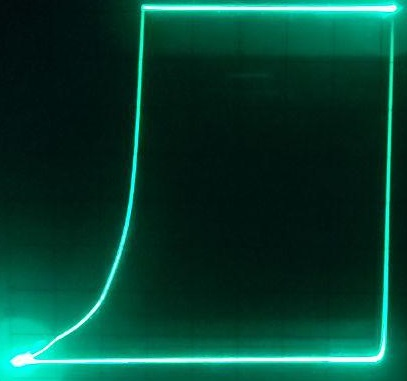
\includegraphics[width=\textwidth]{osc_dark_high_e.jpg}
	\caption{XXXXXXXXXXX}
	\label{fig:dark_high}
	\end{subfigure}
	\caption{XXX}\label{fig:hgstuff}
\end{figure}

%1. description of the experimental setup.
%2. Explain how current, accelerating voltage, reverse bias and collector current should fit
%together if the laws of classical physics would apply.
%3. Using quantum mechanics how would you explain the connection between IC and UA.
%Give an account for the values of accelerating voltages for the different maxima and
%minima, present your results in a table. From these values deduce the excitation energy.
%Take great care in your explanation of the experiment. To facilitate your process of
%understanding you can perform an ’gedanken experiment’ like following an electron as
%it is moving from the source to the collector. Ask yourself questions like, where in
%the tube will excitations occur, what happens to the electron after exciting a mercury
%atom, if an electron of constant kinetic energy (like 1eV) would move from the glowing
%filament to the collector how long would this take, how much is this in comparison to
%the time it takes to complete one cycle (at 50Hz).
%4. In your report you should also include an analysis of what happens to the current
%curve if you change the reverse bias, the current in the glowing filament, the maximum
%acceleration voltage and the temperature of the oven.
